\documentclass[10pt]{article}
\usepackage{verbatim}
\usepackage{multirow}
\usepackage{fullpage}
\usepackage{graphicx}

\pagestyle{plain}

\title{{\normalsize CSCI 572: Computer Networks (Fall 2023)}\\Proposal: Ad-Hoc Messaging App}
\author{Michael Alvarez, Luke Beukelman, Ben Breisch}
\date{October 9th 2023}

\begin{document}
\maketitle

\section{Introduction}
% Motivate the problem;
% Define/formulate the problem: assumptions, application requirements, goals and non-goals;
If I want to send a message to my friend in the next room over, it must travel much farther than the distance between us. Messages sent through SMS or Apple's iMessage must travel from the originating device through a series of intermediate infrastructure nodes before reaching the destination device. This is an issue for both latency and network congestion. In an increasingly connected (and congested) world - why bother wasting bandwidth on a message to a nearby device that can be sent directly from peer to peer? We aim to solve this issue by proposing and developing a peer-to-peer messaging app for Android using Wi-Fi Direct for multi-hop ad-hoc networking. Although security is always an issue with wireless communication, that is out of the scope of this project.
\section{Related work}
   %\item What has been done before?
    %\item How does your solution compare to them?
    There are some existing apps available for Android and iOS. Many of these apps use Bluetooth
    https://engage.sinch.com/blog/offline-messaging-apps/ \\
    https://apps.apple.com/us/app/walkie-talkie-p2p/id1181349764 \\
    https://ieeexplore.ieee.org/document/9473791 \\
    https://arxiv.org/abs/1601.00028 \\
    https://github.com/NaniteFactory/Wifi-Direct-on-Linux \\
    https://github.com/tigewilliams/WifiDirect
  
\section{Approach} %(optional)
%    \item Rationale: Why is it a good idea?
   %     \item Sketch of your approach and design.
   Mobile app development, especially for Android, has an extremely wide range of resources on the Internet. The Android platform is well supported by the community and we plan to leverage online reousrces for the development of this app. For our mobile app to function properly, we will need mock ups of different pages and screens. In the User Interface / User Experience (UI/UX) industry, these are called wireframes. We have created two wireframes, each showing the sign-in page and the messaging page of the application respectively. The wireframes were created in a free tool called WonderShare and are shown in the image below. \\
   \begin{center}
   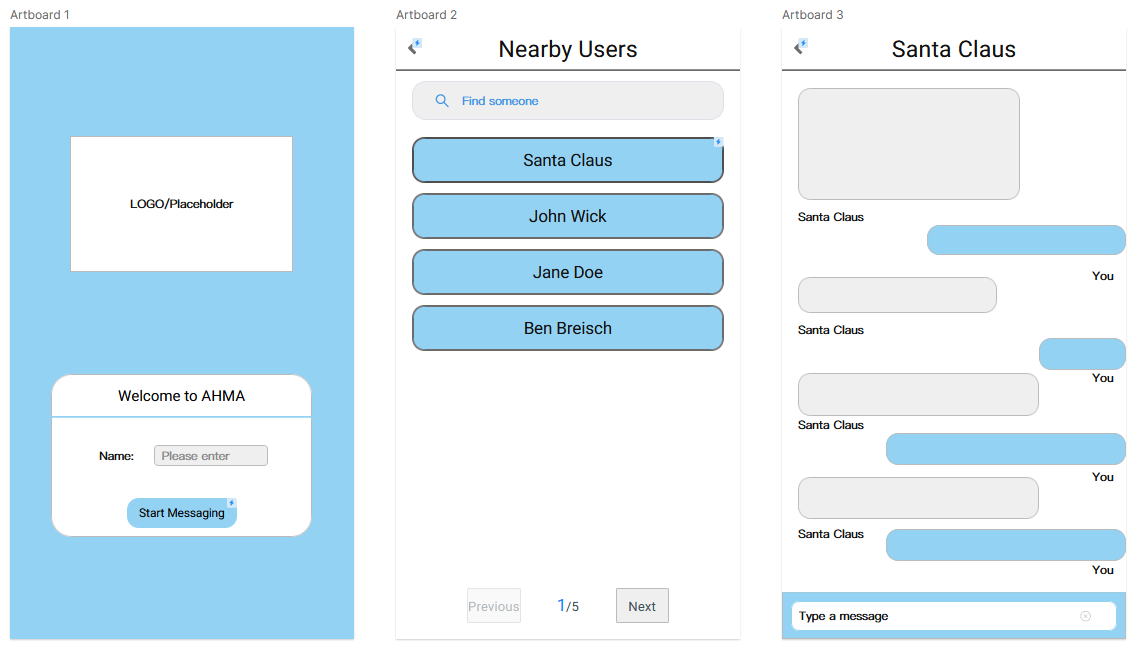
\includegraphics[scale=0.5]{wireframe.png} \\
   \end{center}
   Behind the scenes, this application will use a complex set of functions and internal storage structures. Devices will periodically broadcast beacon frames with routing information, tagged with usernames for each device. This technique is essentially a fusion of AODV and DSDV routing. When the app is open on a device, it will listen for these beacon frames and update its routing table accordingly. If a device receives a frame destined for a different host, it will look up the host in its routing table and determine if it is reachable, forwarding the packet along if it is. When a frame is received at the destination host, it will detect errors with a checksum or CRC32 and reply with an ACK. Messages will be limited to 1024 characters in order to cut down on network latency and reduce packet loss. Conversations between users will be stored on the device.
   
\section{Evaluation Plan}
%      \item What experiments are you going to run?
   %   \item What criteria and metrics are you going to use to evaluate your solutions?
   Criteria:
    
\section{Milestones} %(with dates)
The table below describes the milestones and associated due dates for each.
\begin{center}
\begin{tabular}{ |c|c|c| }
\hline
 Milestone & Explanation \\ \hline
 Install Development Tools &  Oct 14, 2023 \\
 Initial Implementation & Oct 21, 2023 \\
 Begin Final Report Writing & Nov 1, 2023 \\ 
 Finish App Implementation & Nov 15,2023 \\
 Final Report Due & Nov 22, 2023   \\
 \hline
\end{tabular}
\end{center}

\bibliographystyle{plain}
\bibliography{yourref.bib}


\end{document}
